\documentclass[11pt,aspectratio=1610,xcolor=dvipsnames]{beamer}

\usetheme[
    background=light,
    numbering=fraction,
    block=fill,
    progressbar=frametitle
]{metropolis}

\graphicspath{{img/}}

\usepackage[style=authortitle-ibid,backend=biber]{biblatex}
\addbibresource{refs.bib}
\setbeamerfont{footnote}{size=\scriptsize}
% \setbeamercovered{transparent}

\usepackage{physics}
\usepackage{mathtools}
\usepackage{bbm}
\usepackage{booktabs}
\usepackage[most,skins,theorems]{tcolorbox}
\tcbset{variables/.style={colback=yellow!20,colframe=yellow}}
\usepackage{tikz}
\usetikzlibrary{shapes.geometric, arrows, shadows}
\usetikzlibrary{fit, backgrounds}



% \colorlet{LightLavender}{Lavender!40!}
\newtcolorbox{prob}{colback=red!5!white,colframe=red!75!black}
\usefonttheme[onlymath]{serif}
\usepackage{quantikz}
\usepackage{qrcode}
\usepackage{pgfplots}
\usepackage{pythonhighlight}

\newcommand{\R}{\mathbb{R}}
\newcommand{\e}{\mathrm{e}}
\newcommand{\U}[1]{\mathsf{U}(#1)}
\newcommand{\defeq}{\stackrel{\text{\tiny def}}{=}}

\titlegraphic{
\includegraphics[width=0.3\textwidth]{unitary_fund_logo.png}}

\title{Locality and Error Mitigation of Quantum Circuits}
\subtitle{Quantum Wednesday}
\date{Apr 19, 2023}
\author{Nate Stemen}


\begin{document}

\maketitle

\begin{frame}{Today's Paper}
	\begin{figure}[h]
		\centering
		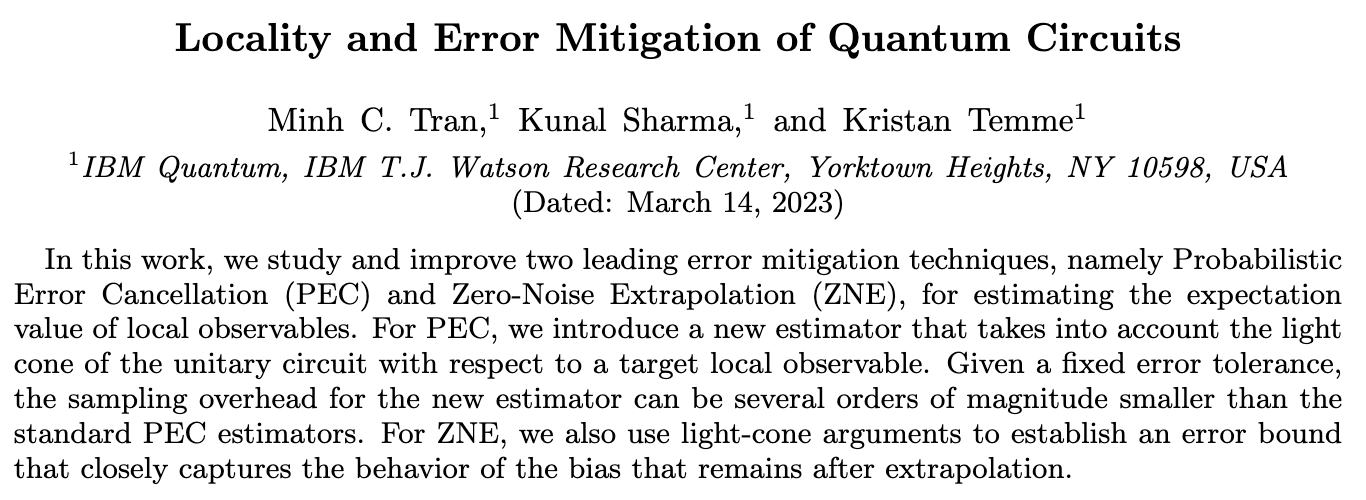
\includegraphics[width=0.8\textwidth]{paper.png}
	\end{figure}
	\begin{center}
		\url{https://arxiv.org/abs/2303.06496}
	\end{center}
\end{frame}

\begin{frame}{Review\footcite{zne-pec}}
	\begin{columns}
		\begin{column}[T]{0.5\textwidth}
			\uncover<+->{{\Large Zero-Noise Extrapolation}}
			\uncover<+->{\begin{center}
					\includegraphics[width=0.9\textwidth]{zne_workflow}
				\end{center}
			}
			\uncover<+->{
				\begin{itemize}
					\item $\expval{A(\lambda)} = \tr\!\qty[A \rho(\lambda)]$
					\item biased estimator, but \emph{no knowledge} of noise model needed
					\item error bounded by (Richardson) extrapolation error
				\end{itemize}
			}
		\end{column}
		\uncover<+->{
			\begin{column}[T]{0.5\textwidth}
				{\Large Probabilistic Error Cancellation}
				\uncover<+->{\begin{center}
						\includegraphics[width=0.86\textwidth]{pec_workflow}
					\end{center}
				}
				\uncover<+->{
					\begin{itemize}
						\item $\expval{A} = \tr\!\qty[A \, \mathcal{U}(\rho)] = \sum\limits_{\vec{\alpha}} \eta_{\vec{\alpha}} \expval{A_{\vec{\alpha}}}_\text{noisy}$
						\item \emph{unbiased} estimator, but requires detailed knowledge of noise model
						\item more efficient methods exist\footnotemark
					\end{itemize}
				}
			\end{column}
		}
	\end{columns}
	\footcitetext{automated-per}
\end{frame}

\begin{frame}{Probabilistic Error Cancellation}
	\only<1>{
		\begin{center}
			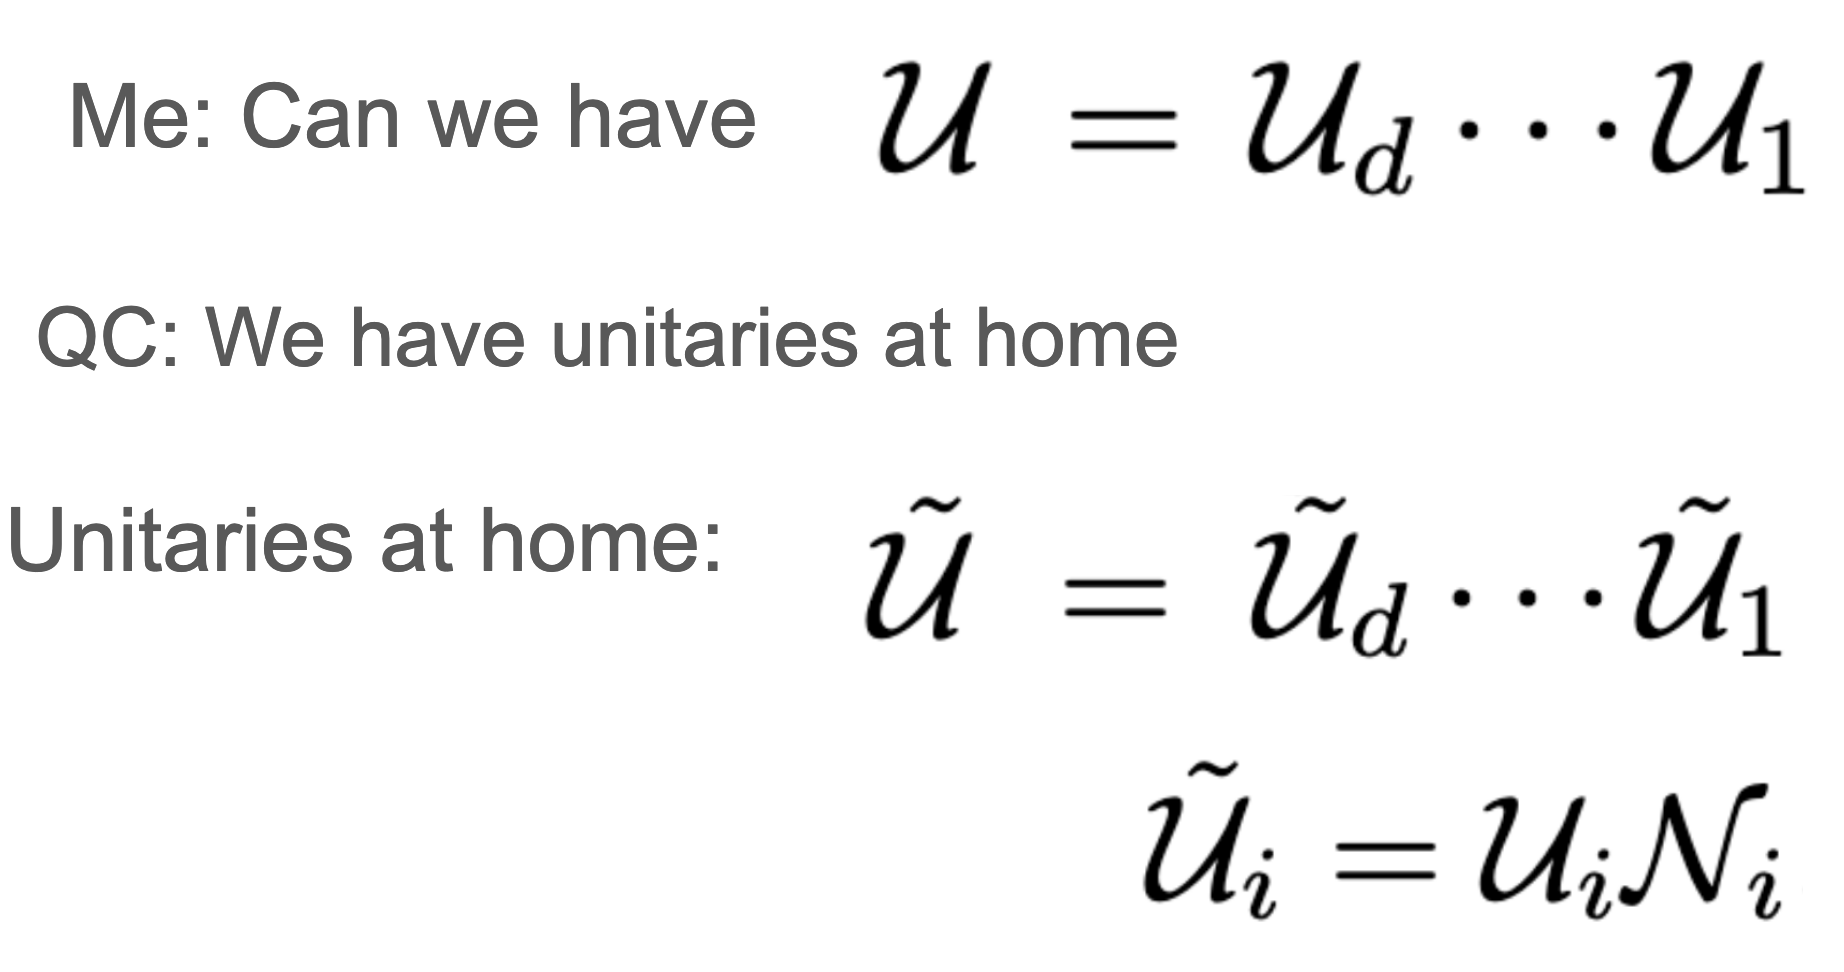
\includegraphics[width=0.9\textwidth]{unitaries-at-home}
		\end{center}
	}
	\only<2->{
		\begin{enumerate}[<+->]
			\item $\tilde{\mathcal{U}} = \tilde{\mathcal{U}}_d \cdots \tilde{\mathcal{U}}_1$ with $\tilde{\mathcal{U}}_i = \mathcal{U}_i \mathcal{N}_i$
			\item Write noise as $\mathcal{N}_i = \e^{\mathcal{L}_i}$ where $\mathcal{L}_i(\rho) = \sum_{j = 1}^J \lambda_{ij}\qty(P_{ij}\rho P_{ij}^\dag - \rho)$
			\item Factorize $\mathcal{N}_i = \prod_{j = 1}^J \mathcal{N}_{ij}$ where $\mathcal{N}_{ij} = (1 - p_{ij})\rho + p_{ij}P_{ij}\rho P_{ij}^\dag$
			\item $\tilde{\mathcal{U}} = \prod_{i = 1}^d \mathcal{U}_i \prod_{j = 1}^J \mathcal{N}_{ij}$
			\item $\tilde{\mathcal{U}}_\text{PEC} = \prod_{i = 1}^d \tilde{\mathcal{U}}_i \qty(\prod_{j = 1}^J \mathcal{N}_{ij}^{-1})$
			\item Probabilistically implement $\mathcal{N}_{ij}$ by applying $P_{ij}$ before $\tilde{\mathcal{U}}_i$ with probability $p_{ij}$
		\end{enumerate}
	}
\end{frame}

\begin{frame}{Key Concepts}
	\begin{columns}
		\begin{column}[t]{0.5\textwidth}
			{\Large Local Observable}
			\begin{enumerate}
				\item An \emph{observable} is a thing that we can design an experiment to measure.
				\item Mathematically, this means a self-adjoint, or Hermitian, operator $A = A^\dag$.
				\item \textbf{Local} means $A$ is supported one a subset of the quantum systems at hand.
				\item Examples:
			\end{enumerate}
		\end{column}
		\uncover<2->{
			\begin{column}[t]{0.5\textwidth}
				{\Large Light Cone}
				\begin{center}
					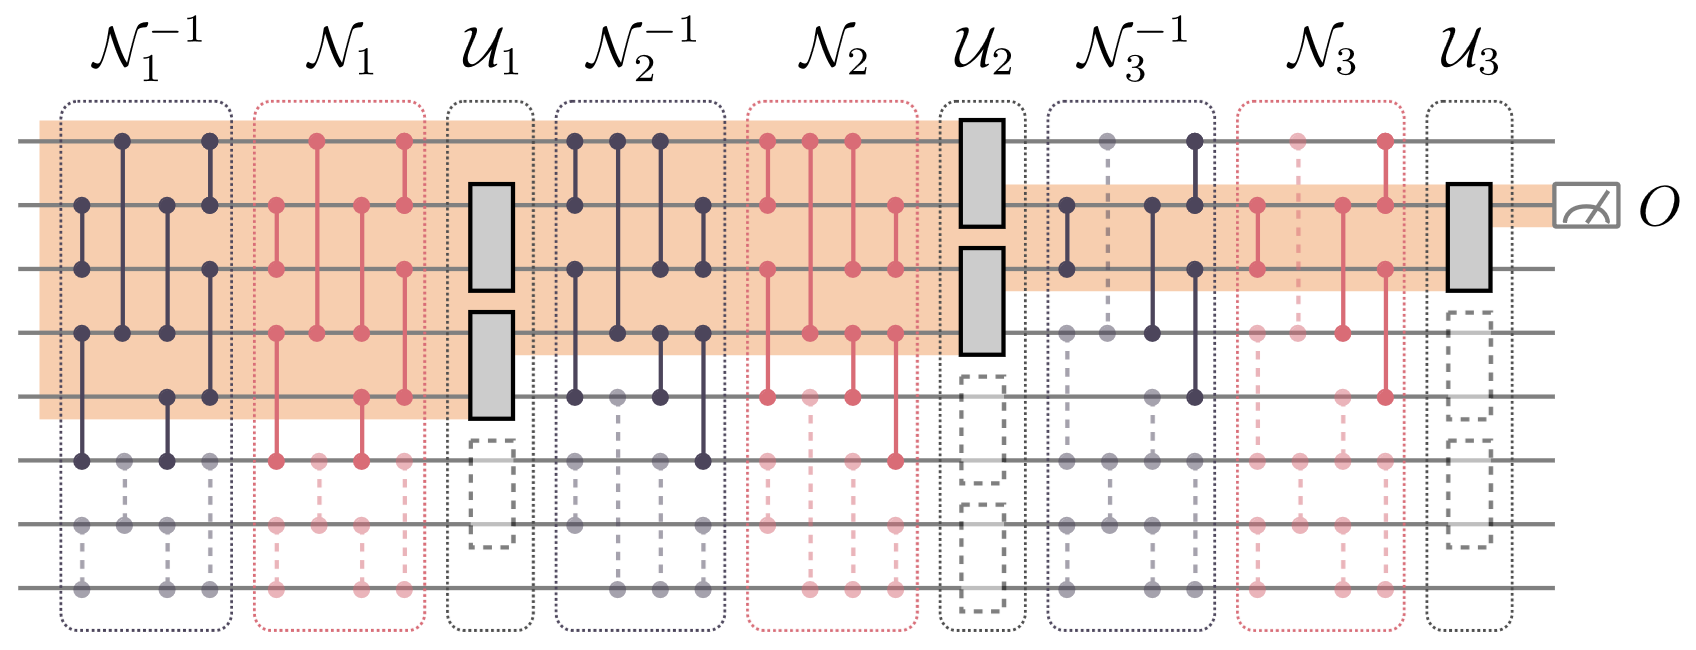
\includegraphics[width=\textwidth]{lightcone}
				\end{center}
				\begin{enumerate}
					\item $\mu_i = \operatorname{supp}\!\qty(\mathcal{U}_i^\dag\mathcal{U}_{i+1}^\dag\cdots\mathcal{U}_d^\dag(O))$
				\end{enumerate}
			\end{column}
		}
	\end{columns}
\end{frame}

\begin{frame}{PEC Results}
	\begin{table}[h]
		\centering\begin{tabular}{c | c}
			Unlocal                                                                                                         & Local                                                                                                                            \\ \toprule
			$\hat{o}_z^\text{PEC}(\boldsymbol{\sigma}) = o_z(\boldsymbol{\sigma})\prod\limits_{i, j}\gamma_{ij}\sigma_{ij}$ & $\hat{o}_z^\text{LoPEC}(\boldsymbol{\sigma}) = o_z(\boldsymbol{\sigma})\prod\limits_{(i, j) \in \mu} \gamma_{i, j}\sigma_{i, j}$ \\
			$\operatorname{Var}\!\qty[\hat{o}_z^\text{PEC}] = \order{\exp[4\sum_{i,j}\lambda_{ij}]}$                        & $\operatorname{Var}\!\qty[\hat{o}_z^\text{LoPEC}] = \order{\exp[4\sum_{(i, j) \in \mu}\lambda_{i, j}]}$
		\end{tabular}
	\end{table}
	\uncover<2->{
		\only<2>{
			\begin{center}
				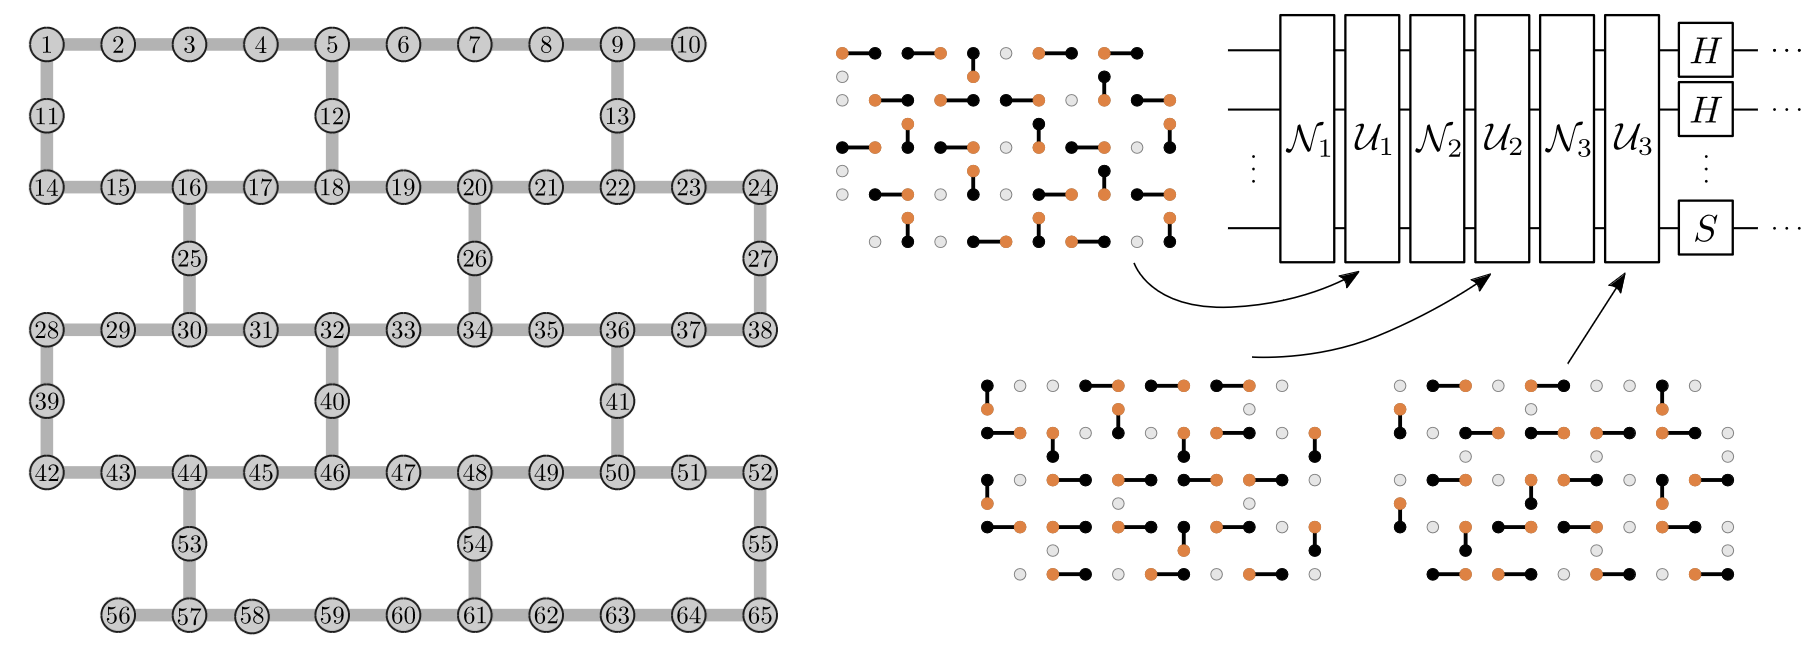
\includegraphics[width=0.9\textwidth]{numerical-setup}
			\end{center}
		}
		\only<3>{
			\begin{center}
				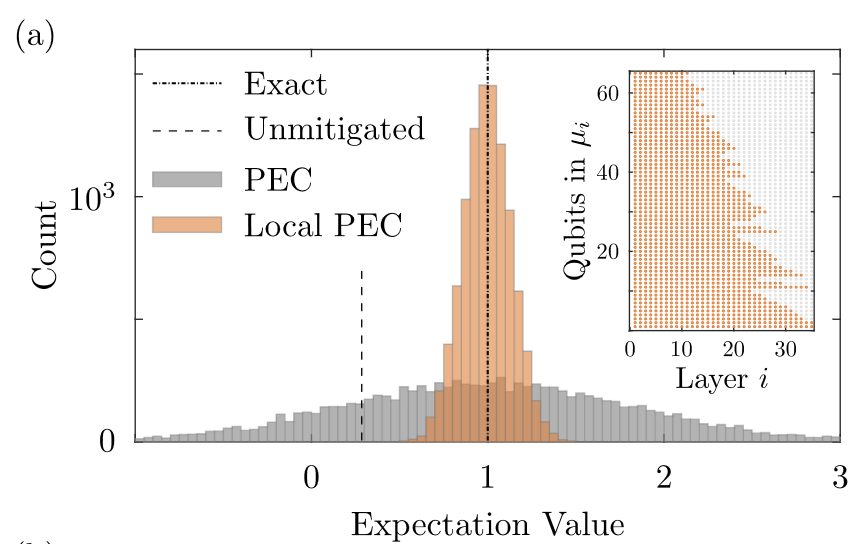
\includegraphics[width=0.49\textwidth]{distribution}
				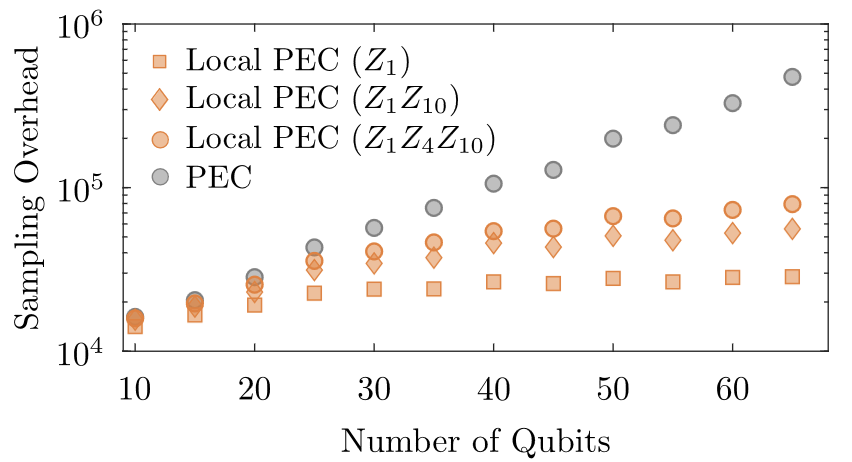
\includegraphics[width=0.5\textwidth]{overhead}
			\end{center}
		}
	}
\end{frame}

\begin{frame}{ZNE Results}
	\begin{center}
		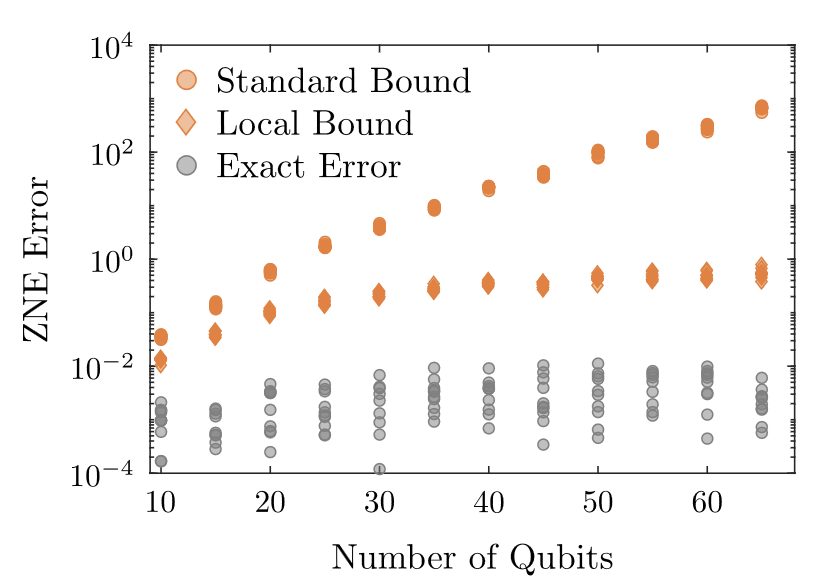
\includegraphics[width=0.6\textwidth]{zne-bounds}
	\end{center}
\end{frame}

% \begin{frame}{PEC Results}
% 	\only<1>{
% 		\begin{center}
% 			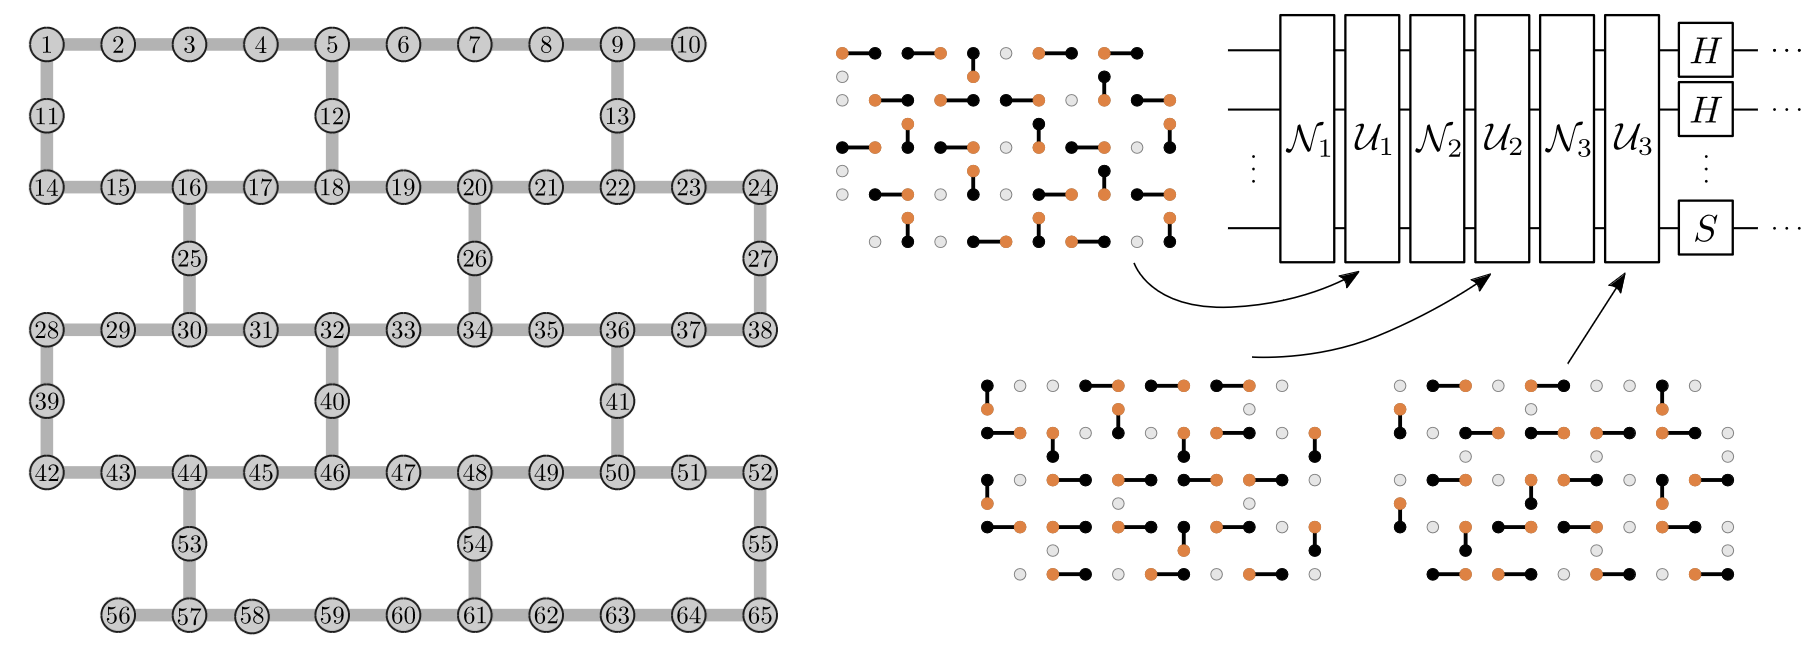
\includegraphics[width=0.9\textwidth]{numerical-setup}
% 		\end{center}
% 	}
% 	\only<2>{
% 		\begin{center}
% 			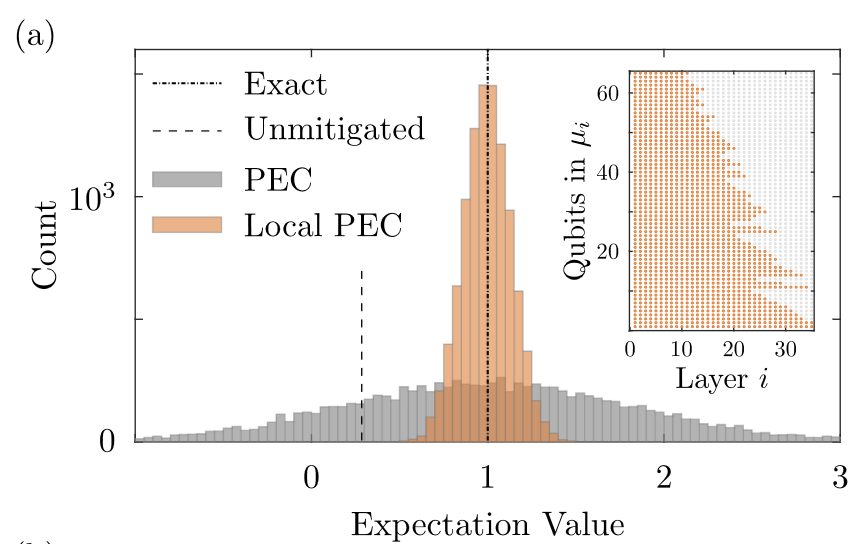
\includegraphics[width=0.49\textwidth]{distribution}
% 			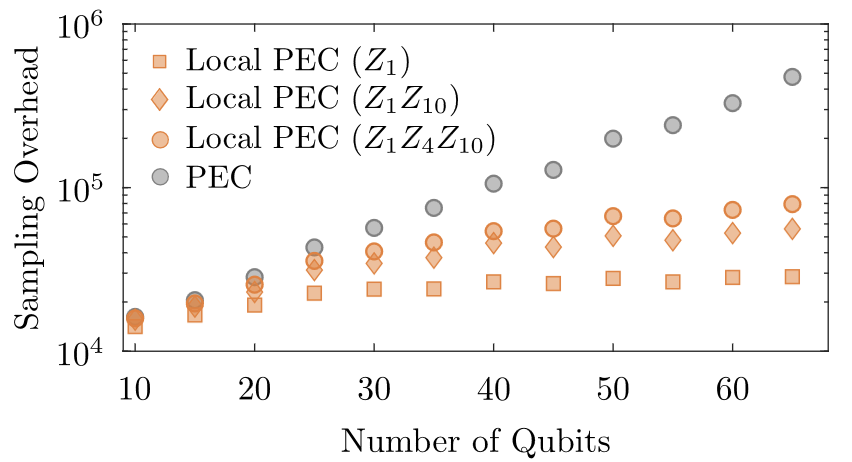
\includegraphics[width=0.5\textwidth]{overhead}
% 		\end{center}
% 	}
% \end{frame}

\begin{frame}[fragile]{Questions}
	\begin{enumerate}
		\item Does this slot into our existing \verb|execute_with_pec| function?
		\item How does this perform as an observable $O$ go from local to ``unlocal''.
		\item Are the assumptions (efficiently learned)
	\end{enumerate}
\end{frame}

\begin{frame}{and then\dots}
	\begin{center}
		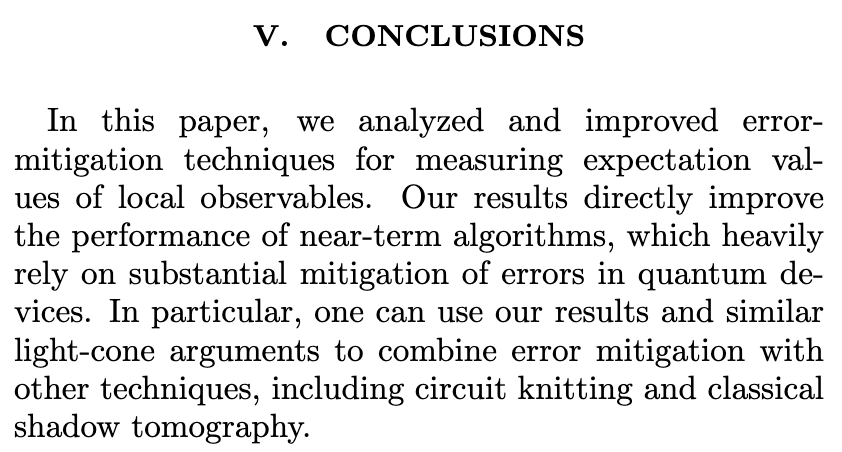
\includegraphics[width=0.7\textwidth]{lookahead}
	\end{center}
\end{frame}

\begin{frame}[standout]
	Thank you!
\end{frame}

\end{document}
